%File: formatting-instruction.tex
\documentclass[letterpaper]{article}
\usepackage{url,graphicx,xcolor}
\usepackage{times}
\usepackage{helvet}
\usepackage{courier}
\usepackage{booktabs}
\usepackage{siunitx}
\usepackage[guidelines]{faikrmod3}
% \usepackage[]{faikrmod3} % without guidelines
\frenchspacing
\setlength{\pdfpagewidth}{8.5in}
\setlength{\pdfpageheight}{11in}



% THE \pdfinfo /Title AND /Author ARE NOT NECESSARY, THEY ARE METADATA FOR THE FINAL PDF FILE
\pdfinfo{
/Title (Insert Your Title Here)
/Author (Andrea Cristiano)}
\setcounter{secnumdepth}{0}  
\begin{document}
% The file aaai.sty is the style file for AAAI Press 
% proceedings, working notes, and technical reports.
%
\title{Comparison between a Bayesian Network based soccer predictive model and 538 soccer prediction model}
\author{Andrea Cristiano\\
Master's Degree in Artificial Intelligence, University of Bologna\\
andrea.cristiano@studio.unibo.it
}
\maketitle




\begin{abstract}
\begin{quote}

This study compares the predictive performance of a Bayesian Network based model developed for soccer match outcome prediction against the established 538 soccer prediction system. Using historical match data sourced from 538, our model is trained on team statistics and match conditions to forecast match outcomes. We evaluate the accuracy  of our model in comparison to 538's predictions, highlighting the comparable outcomes of the two models.


\end{quote}
\end{abstract}


\section{Introduction}
\subsection{Domain}

In the realm of soccer analytics, one of the most studied and relevant areas consists in the prediction of the outcome of each match. In this project we are going to introduce a Bayesian Network model to predict matches whose structure is inspired by some of the Bayesian Network approaches already present in the literature (such as ~\cite{article1} \cite{BayesianBarca}) and by FiveThirtyEight(538) own soccer prediction algorithm, one of the most relevant and well known models in this class \cite{538Website}.


\subsection{Aim}

The aim of this project is to analyse the performances of a Bayesian Network based model to predict the result of soccer matches to see if an approach of this kind is useful and reliable for the task.


\subsection{Method}

To train and test the model we used 538's own database (available at \cite{538DB}) in order to make the comparison between the two models as reliable as possible. \ The Bayesian Network model was implemented trough the \textit{pgmpy} library and the inference steps were performed trough Variable Elimination. Since \textit{pgmpy} requires the discretization of the values it operates with, we performed the discretization process over three columns of the dataset, which are going to be the input values of our model. To improve the accuracy of the model, for each one of the columns involved, we tested different values for the discretization number.


\subsection{Results}



We observed that the accuracy of the Bayesian model is comparable to the accuracy of 538's model, for some leagues the accuracy of the custom model is slightly better than 538's, while on others is slightly worse.



\section{Model}

%
\begin{figure}
    \centering
    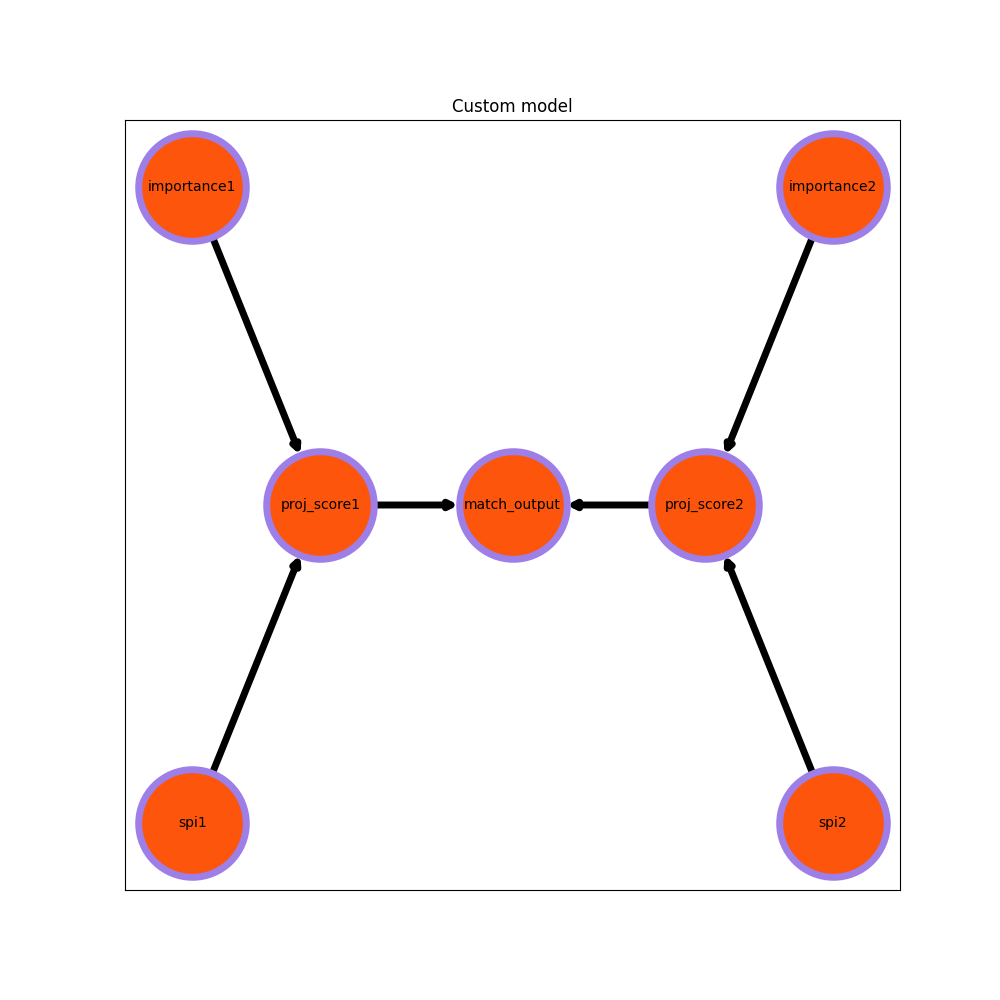
\includegraphics[scale=0.4]{images/bayesian_model.png}
    \caption{Custom Bayesian Model }
    \label{fig:network}
\end{figure}

\begin{figure*}[t]
    \centering
    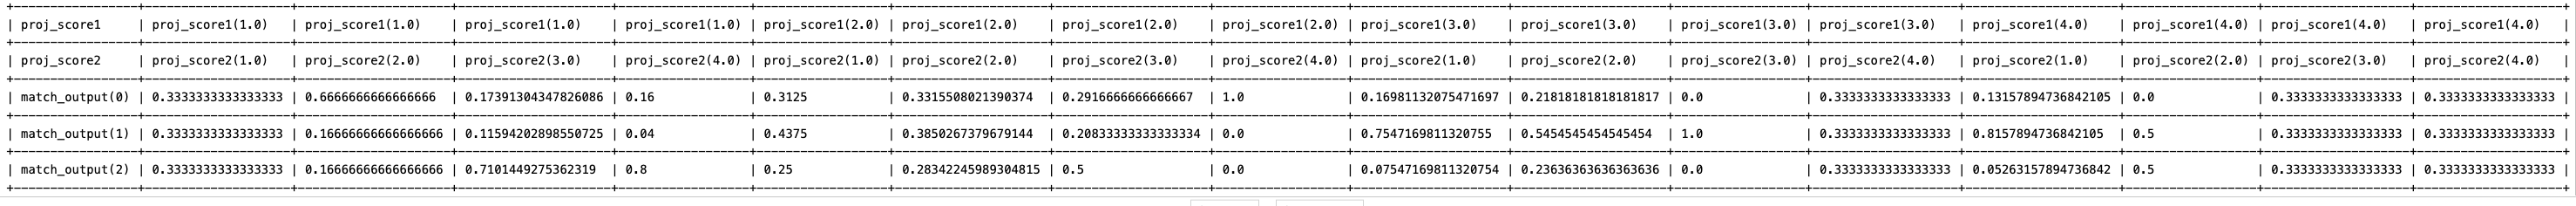
\includegraphics[scale=0.35]{images/Cpt.png}
    \caption{Conditional Probability Table for Match\_output }
    \label{fig:network}
\end{figure*}


The model is composed by 7 nodes in total: 3 for each team and 1 dedicated to the output. The semantic of the nodes is the following:
\begin{itemize}
    \item Importance: How important is the match for the team in that specific moment of the season, how influential the outcome is on the standings.
    \item Spi: it is a measure of the team overall strength.
    \item Proj\_score: is the projection of the amount of goals we predict each team is going to score given its overall strength and the importance of the match.
    \item Match Output: it has 3 values describing the probabilities for each possible outcome (0 for draw, 1 for home win, 2 for away win).

\end{itemize}

Looking at the CPT we can observe that, if the difference between the proj\_score of the two teams is significant, then the probabilities in the CPT will reflect that. We also observe that for some combinations the probabilities are distributed evenly. 


The structure of the model is based on the basic structure that also 538 uses \cite{538Website}: we use the same input parameters and with those we calculate the projected score, which will, in the end, determine the probability distribution of the output. This allows us to better understand how much the kind of model uses influences the results. 



\section{Analysis}

\subsection{Experimental setup}

The model has been trained over the seasons 2020-2021, 2021-2022, 2022-2023. The test set is made of the games after the matchday 20. This choice has been made in order to have a sufficient amount of matches to train the model on.


For each match into the test set we took as the model's best guess the proposed outcome of the match whose probability were the highest: we then compared the predicted outcome against the actual outcome. We calculated the accuracy based upon the number of correct guesses the model has made over the total number of match considered. 

The inference steps were performed trough Variable Elimination: for each match only the importance and the spi of the two teams were given as an input.


\subsection{Results}

We observed that the model overperforms 538's model in predicting the outcome of Serie A matches and Spanish La Liga, while slightly underperforms 538's in Premier League, League 1, and German Bundesliga.  The results satisfy the initial expectations.



\begin{figure}
    \centering
    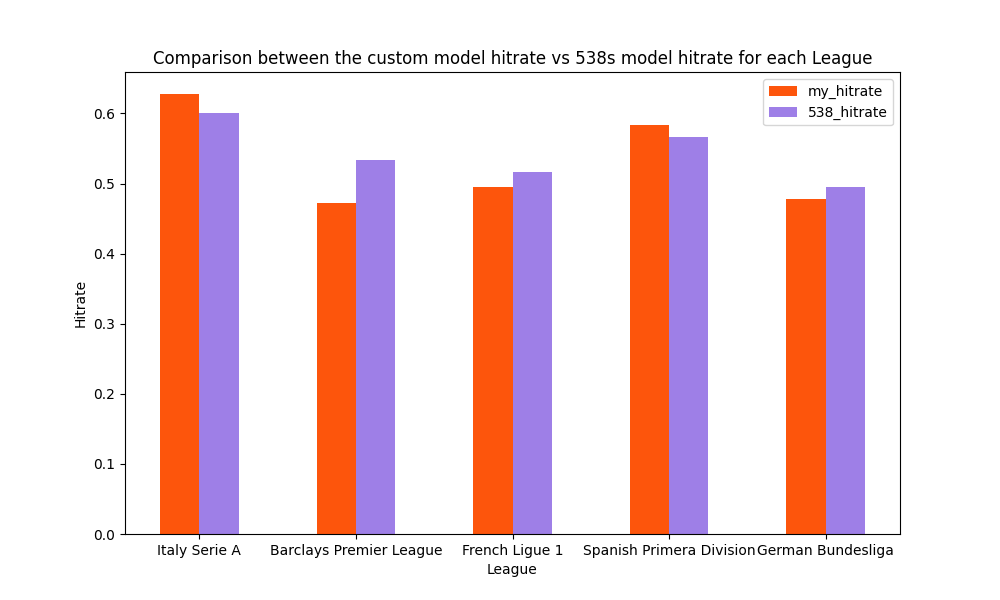
\includegraphics[scale=0.35]{images/comparison.png}
    \caption{Accuracy comparison between the two models on Europe's top 5 leagues }
    \label{fig:network}
\end{figure}





\section{Conclusion}

In this project we explored the usage of Bayesian Networks as a models to predict soccer matches outcomes. We observed that, using the best combination of parameters, the model returns promising results, averaging an accuracy close to a well-known prediction model.

We can then conclude that Bayesian Networks could be a valuable tool to predict soccer matches outcomes.


\section{Links to external resources}

\begin{itemize}
    
    \item 538 soccer dataset:  \url {https://github.com/fivethirtyeight/data/tree/master/soccer-spi}
\end{itemize}


\bigskip

\bibliographystyle{aaai}
\bibliography{faikrmod3.bib}


\end{document}